\documentclass[11pt,a4paper]{article}

\usepackage[utf8]{inputenc}
\usepackage[T1]{fontenc}
\usepackage{lmodern}
\usepackage[spanish]{babel}
\usepackage[margin=1in]{geometry}
\usepackage{amsmath,amssymb}
\usepackage{booktabs}
\usepackage{graphicx}
\usepackage{hyperref}
\usepackage{tcolorbox}
\tcbuselibrary{listings}

\newtcblisting{rcode}{
    listing only,
    colback=gray!5,
    colframe=gray!20,
    boxrule=0.4pt,
    sharp corners,
    listing options={
        language=R,
        basicstyle=\ttfamily\footnotesize,
        breaklines=true,
        showstringspaces=false,
        literate=
            {á}{{\'a}}1 {é}{{\'e}}1 {í}{{\'{\i}}}1 {ó}{{\'o}}1 {ú}{{\'u}}1
            {Á}{{\'A}}1 {É}{{\'E}}1 {Í}{{\'I}}1 {Ó}{{\'O}}1 {Ú}{{\'U}}1
            {à}{{\`a}}1 {è}{{\`e}}1 {ì}{{\`\i}}1 {ò}{{\`o}}1 {ù}{{\`u}}1
            {À}{{\`A}}1 {È}{{\`E}}1 {Ì}{{\`I}}1 {Ò}{{\`O}}1 {Ù}{{\`U}}1
            {ñ}{{\~n}}1 {Ñ}{{\~N}}1 {ç}{{\c c}}1 {Ç}{{\c C}}1
            {ü}{{\"u}}1 {Ü}{{\"U}}1
    }
}

\title{Sesión 1 : Estadística Básica}
\author{
    Daniel Fuertes\\
    %\texttt{student1@example.com}
    \and
    Oscar Moreno\\
    %\texttt{student2@example.com}
    \and
    Marc Torres\\
    %\texttt{student3@example.com}
}
\date{\today}

\begin{document}

\maketitle

\begin{tcolorbox}[colback=gray!20,colframe=gray!20, sharp corners]
1. Calcular la media, la mediana, la desviación tipo, el primer cuartil, el tercer cuartil, el rango intercuartílico y dibujar el correspondiente boxplot de la muestra de datos.
\[ x = (7,80,\ 8,25,\ 12,60,\ 13,50,\ 15,96,\ 16,46,\ 31,29) \]
\end{tcolorbox}

\noindent\begin{minipage}[c]{0.7\textwidth}
\begin{align*}
&\bar{x}=\frac{1}{7}\sum_{i=1}^{7}x_i=15,12\ ; \qquad s=\sqrt{\frac{1}{6}\sum_{i=1}^{7}(x_i-\bar{x})^2}=7,89\\
&x_{(4)}=13,50\ ; \qquad Q_1=x_{(2)}=8,25 \ ;\qquad Q_3=x_{(6)}=16,46\\
&\mathrm{RIC}=Q_3-Q_1=8,21
\end{align*}

\end{minipage}\hfill%
\begin{minipage}[c]{0.2\textwidth}
    \centering
    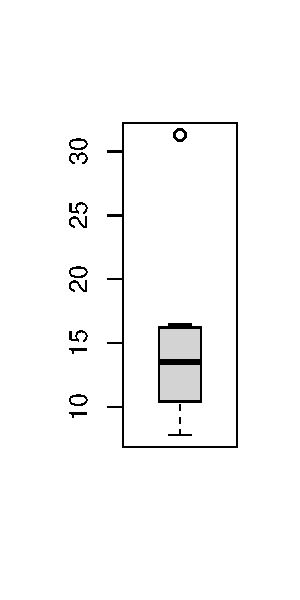
\includegraphics[width=\textwidth,height=5cm,keepaspectratio]{pr1_estad_boxplot1.pdf}
\end{minipage}

\begin{tcolorbox}[colback=gray!20,colframe=gray!20, sharp corners]
2. Justificar que la media de una muestra escogida al azar es un estimador más fiable que la media de una muestra de expertos.
\end{tcolorbox}

No todo el mundo (la población sobre la cual se quiere hacer inferencia) es experto en el sujeto de estudio, por eso la muestra aleatoria es más representativa que una muestra sesgada.

\begin{tcolorbox}[colback=gray!20,colframe=gray!20, sharp corners]
3. Suponga la variable aleatoria “tiempo que tardo en ir de mi casa al trabajo” y diferencie factores sistemáticos y factores aleatorios intervinientes en su medición
\end{tcolorbox}

Un factor sistemático es aquel que desplaza de forma regular el tiempo observado. Por ejemplo, si viajo en autobús, salgo a la hora punta, y empiezo el cronómetro en la puerta, el tiempo suele ser mayor que si viajara en coche, fuera de madrugada y empezara a contar en el portal.
Los aleatorios cambian de un trayecto a otro y su efecto no se conoce de antemano como por ejemplo, los retrasos derivados de la meteorología, una variación del tráfico por un accidente o encontrarse con alguien que detenga el viaje. En distintas mediciones pueden aumentar o reducir el tiempo.

\begin{tcolorbox}[colback=gray!20,colframe=gray!20, sharp corners]
4. Cuando podemos asegurar que el mecanismo generador de una variable aleatoria se aproxima a una distribución gaussiana.
\end{tcolorbox}

Cuando una variable es la suma de muchos efectos aleatorios independientes, con varianzas finitas e igualmente irrelevantes para explicar la misma, su distribución tiende a aproximarse a una distribución normal, por el Teorema Central del Límite.

\newpage 

\begin{tcolorbox}[colback=gray!20,colframe=gray!20, sharp corners]
5. Efectúe un summary de las variables de \texttt{bcn\_pisos.txt}. Detecte si en el fichero proporcionado hay registros duplicados y elimínelos.
\end{tcolorbox}

\begin{rcode}
> summary(pisos)
    Valor              Superf            Dorm           Banys      
 Min.   : 3007368   Min.   : 23.24   Min.   :1.000   Min.   :1.000  
 1st Qu.:12025000   1st Qu.: 64.20   1st Qu.:2.000   1st Qu.:1.000  
 Median :15456000   Median : 78.54   Median :3.000   Median :1.000  
 Mean   :17823727   Mean   : 83.97   Mean   :2.903   Mean   :1.319  
 3rd Qu.:20920248   3rd Qu.: 95.00   3rd Qu.:3.000   3rd Qu.:2.000  
 Max.   :99662144   Max.   :475.30   Max.   :5.000   Max.   :4.000  
                                                                    
      Edat         Estat        Planta               Dist         ValSol      
 Min.   :  0.00   1_MM:395   Atic  : 255   Eixample    :385   Min.   : 20321  
 1st Qu.: 25.00   2_M :692   Bajos : 119   Sant_Marti  :335   1st Qu.:106679  
 Median : 30.00   3_N :856   Planta:1955   Sants       :329   Median :119965  
 Mean   : 40.75   4_B :277                 Horta       :252   Mean   :128708  
 3rd Qu.: 50.00   5_MB:109                 Nou_Barris  :234   3rd Qu.:146537  
 Max.   :289.00                            Ciutat_Vella:192   Max.   :365754  
                                           (Other)     :602                   
  Tipus      Ascens    ExtInt           Reforma   
 BLOQ: 282   NO: 920   EXT:1991   REF1A5    :778  
 MANZ:2047   SI:1409   INT: 338   SINREFORMA:501  
                                  REF5A10   :378  
                                  RECIENREF :197  
                                  REF10-15  :182  
                                  REF>20    :115  
                                  (Other)   :178  
> pisos <- pisos[!duplicated(pisos), ]
\end{rcode}

Hay duplicados porque el que tomó los datos duplicó registros para hinchar la base de datos.

\newpage

\begin{tcolorbox}[colback=gray!20,colframe=gray!20, sharp corners]
6. Represente gráficamente la distribución de cada variable del fichero: histograma o función de densidad para las variables continuas o diagrama de barras para las variables categóricas.
\end{tcolorbox}


\begin{figure}[h!]
 \centering
 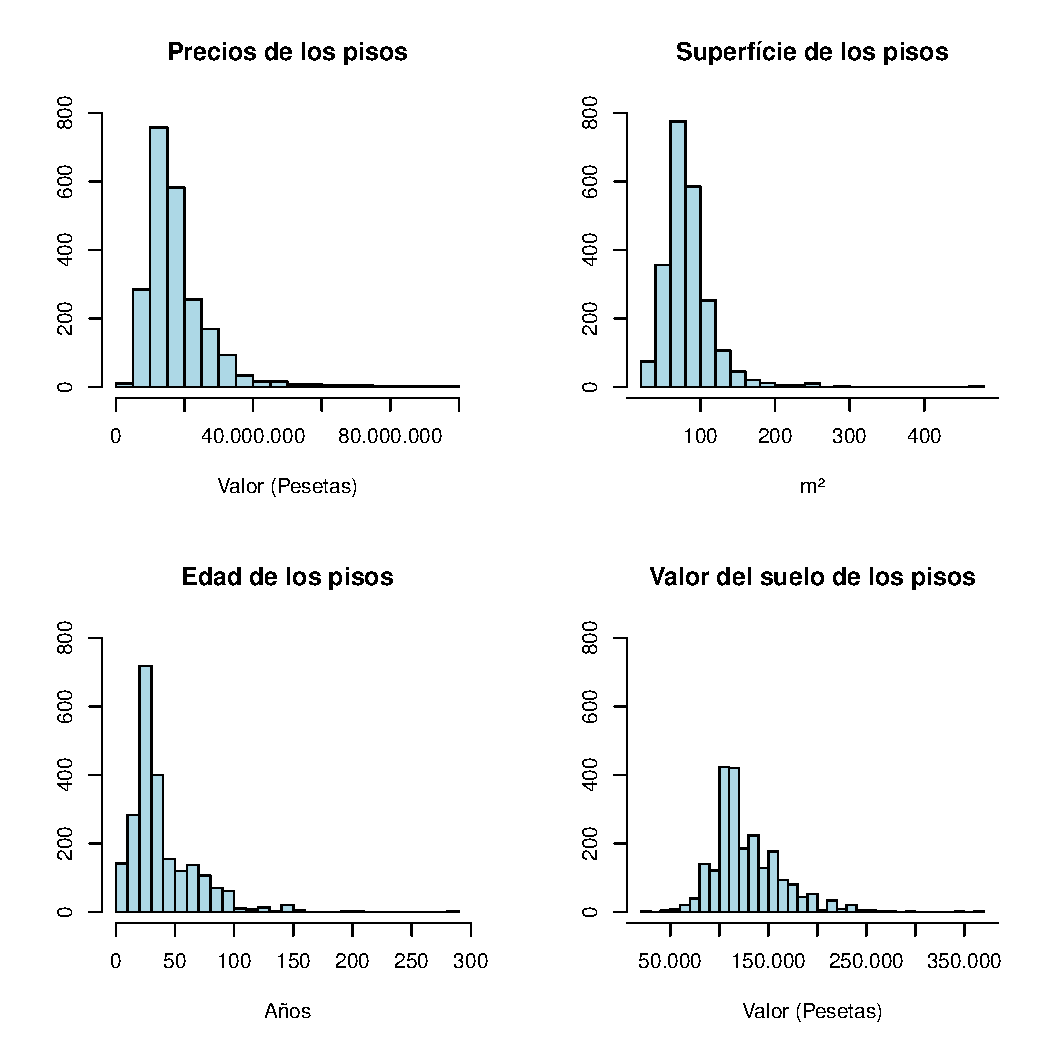
\includegraphics[width = 0.6\linewidth]{pr1_estad_histogramas.pdf}
\end{figure}
\begin{figure}[h!]
 \centering
 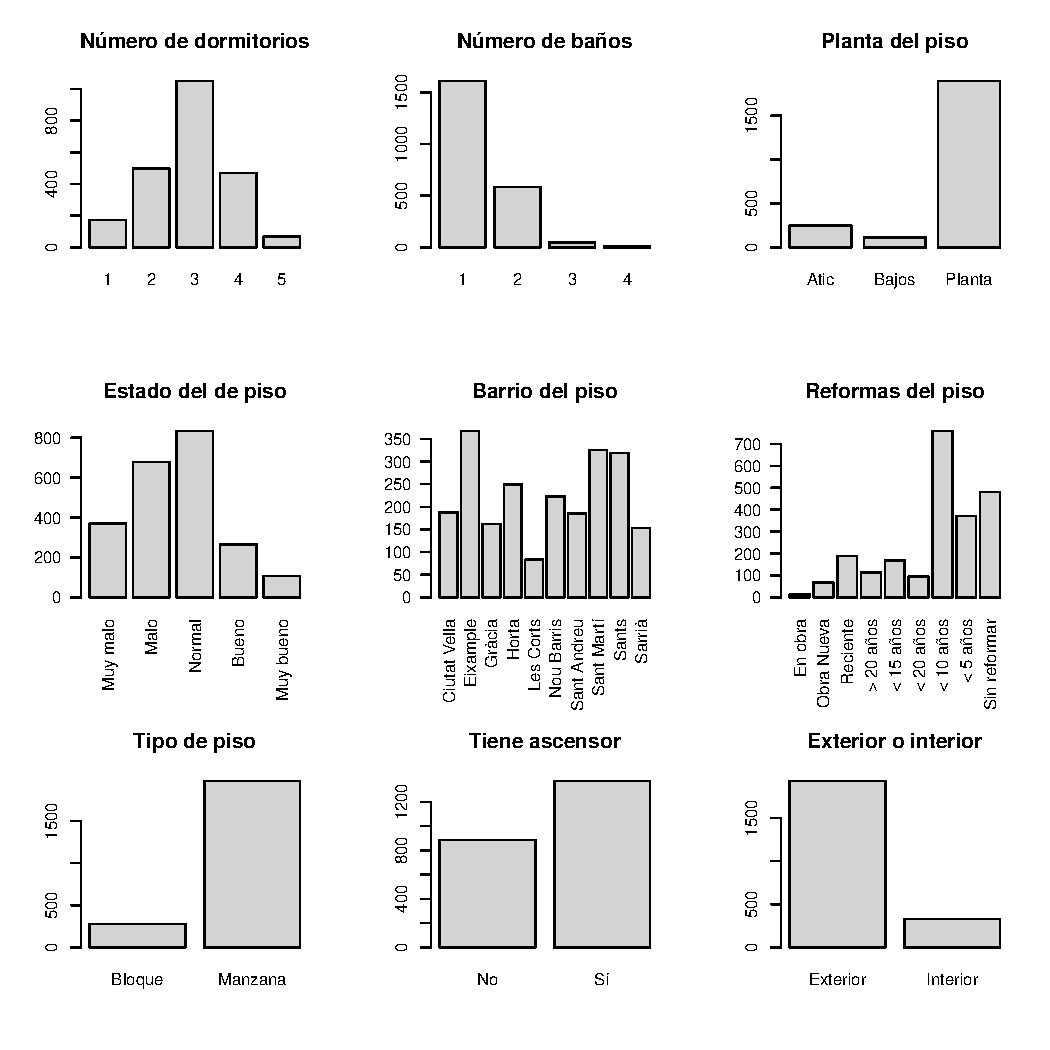
\includegraphics[width = 0.7\linewidth]{pr1_estad_barplots.pdf}
\end{figure}


\begin{tcolorbox}[colback=gray!20,colframe=gray!20, sharp corners]
7. Identifique si existe algún piso que podemos considerar “outlier” (para ello solo tenga en cuenta las variables continuas). Elimínelo del data frame
\end{tcolorbox}

Usamos la función \textit{Local Outlier Factor} de la librería \textit{DescTools} con $k = 5$ sobre las variables contínuas del dataframe pisos.
\begin{rcode}
> outliers.scores <- LOF(scale(pisos_cont), k = 5)
> outlier <- order(outlier.scores, decreasing=T)[1:10]
> cbind(outlier.scores[outliers], pisos_cont[outliers,])
     outlier.scores[outliers]    Valor Superf Edat    ValSol
163                  9.731024  3283200  60.00  198  80107.40
112                  5.966654 80126080 475.30  289 166465.75
162                  2.972040  8450000  65.00  150 100036.25
1787                 2.646105  6908846  86.63   10  20320.85
409                  2.590744 67587904 182.67   60 345825.40
1732                 2.450899 23520000 168.00   35  66821.50
116                  2.383793  7321600  51.20  150  80107.40
1995                 2.306762  7170080  87.44   35  26963.80
1139                 2.287689 38354208 103.66   50 292681.80
1987                 2.265198  6300000  63.00   53  46892.65

\end{rcode}
Viendo estos valores, descartamos los dos primeros, donde podemos ver que su edad es muy elevada, o edad y valor para lo que se esperaría de un piso pequeño. Quizás se trate de pisos históricos con alto valor cultural.


\begin{tcolorbox}[colback=gray!20,colframe=gray!20, sharp corners]
8. Efectúe un diagrama bivariante (plot) entre el “Valor de los pisos” y su “Superficie”. Calcule la covariancia y la correlación entre ambas variables.
\end{tcolorbox}

\begin{figure}[h!]
 \centering
 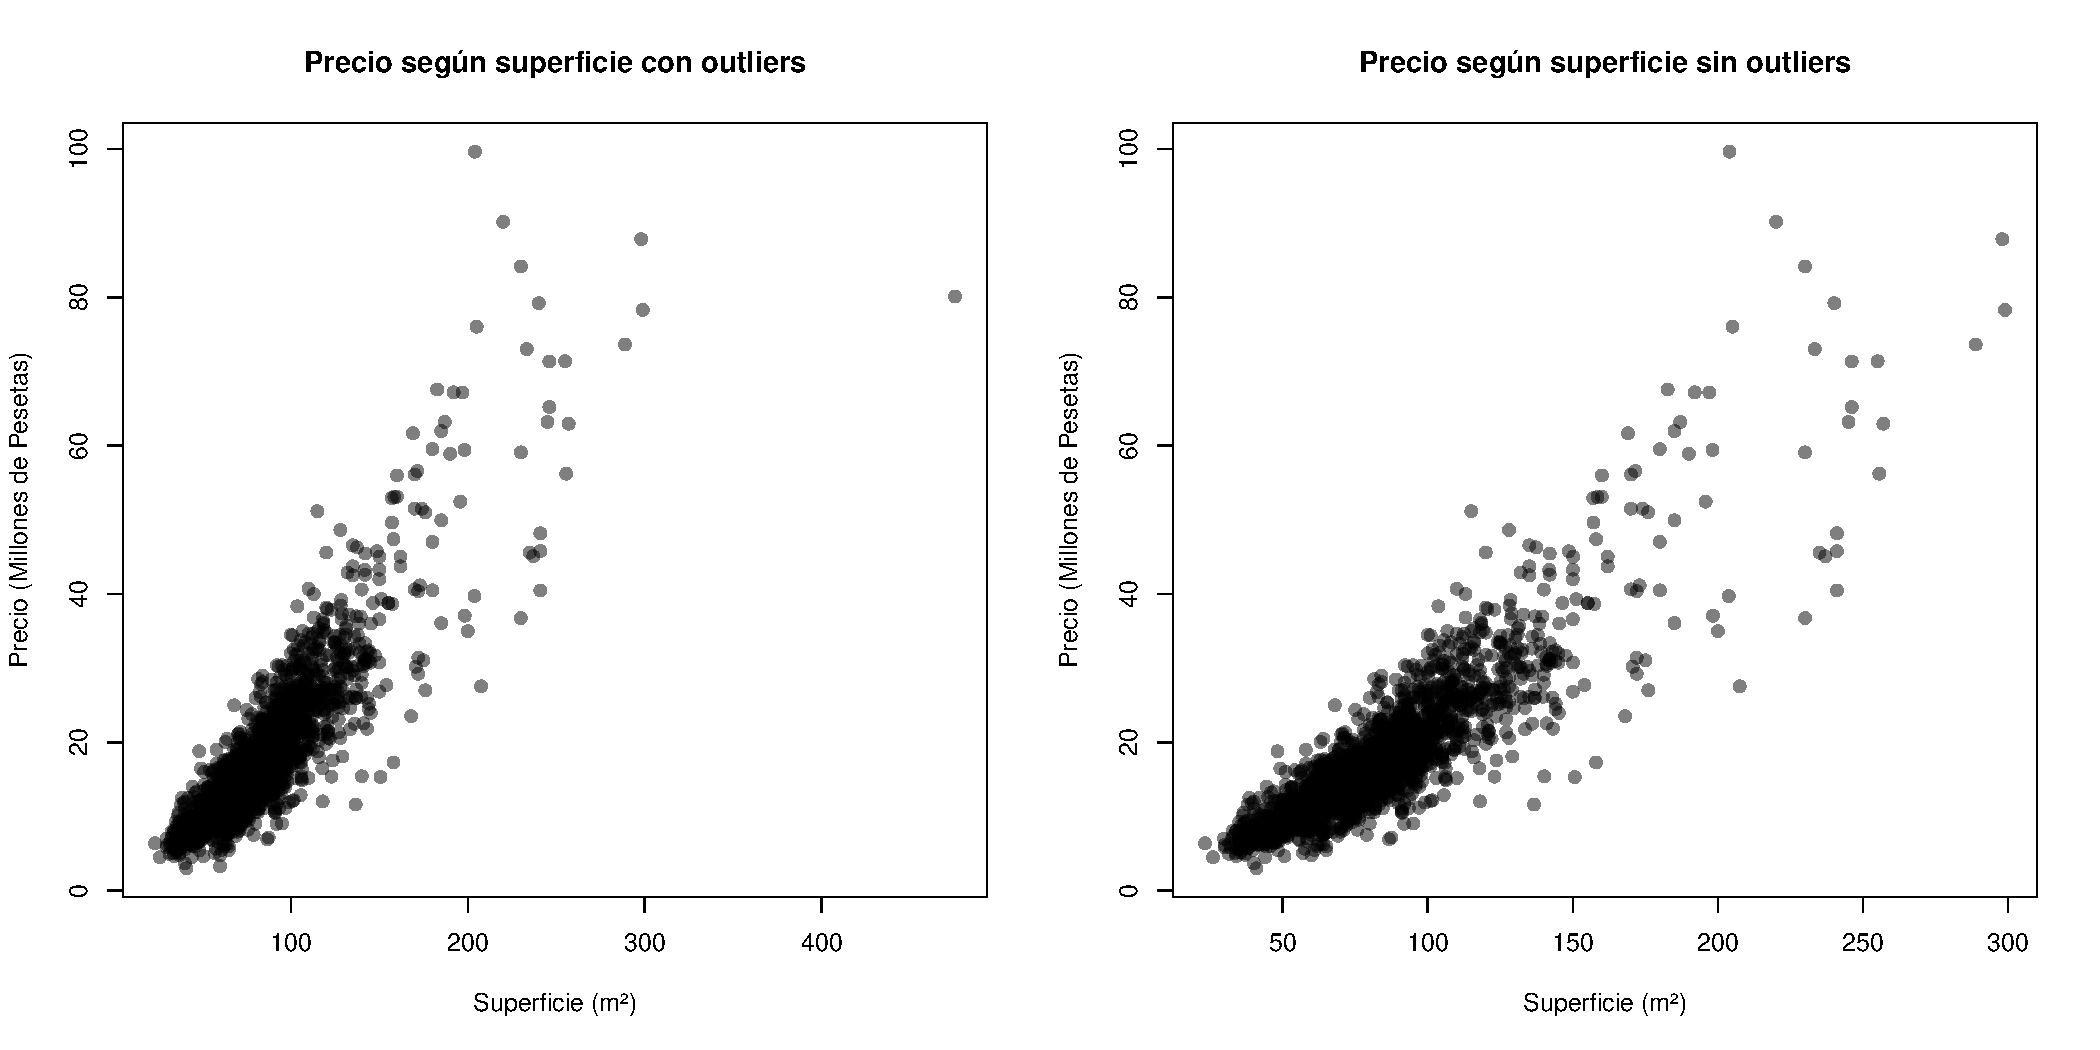
\includegraphics[width = 0.8\linewidth]{pr1_scaterplot1.pdf}
\end{figure}

\begin{rcode}
> cov(pisos_cont_so$Valor, pisos_cont_so$Superf) 
[1] 269332201
> cor(pisos_cont_so$Valor, pisos_cont_so$Superf)
[1] 0.884583
\end{rcode}

Con una covarianza positiva, podemos decir que según incrementa la superfície, incrementa el valor. Con una correlación cercana a 1, decimos que existe una asociación estadística significativa entre ambas variables.

\newpage

\begin{tcolorbox}[colback=gray!20,colframe=gray!20, sharp corners]
9. Calcule la asociación entre el “Valor de los pisos” y el “Distrito”.
\end{tcolorbox}
\begin{figure}[h!]
 \centering
 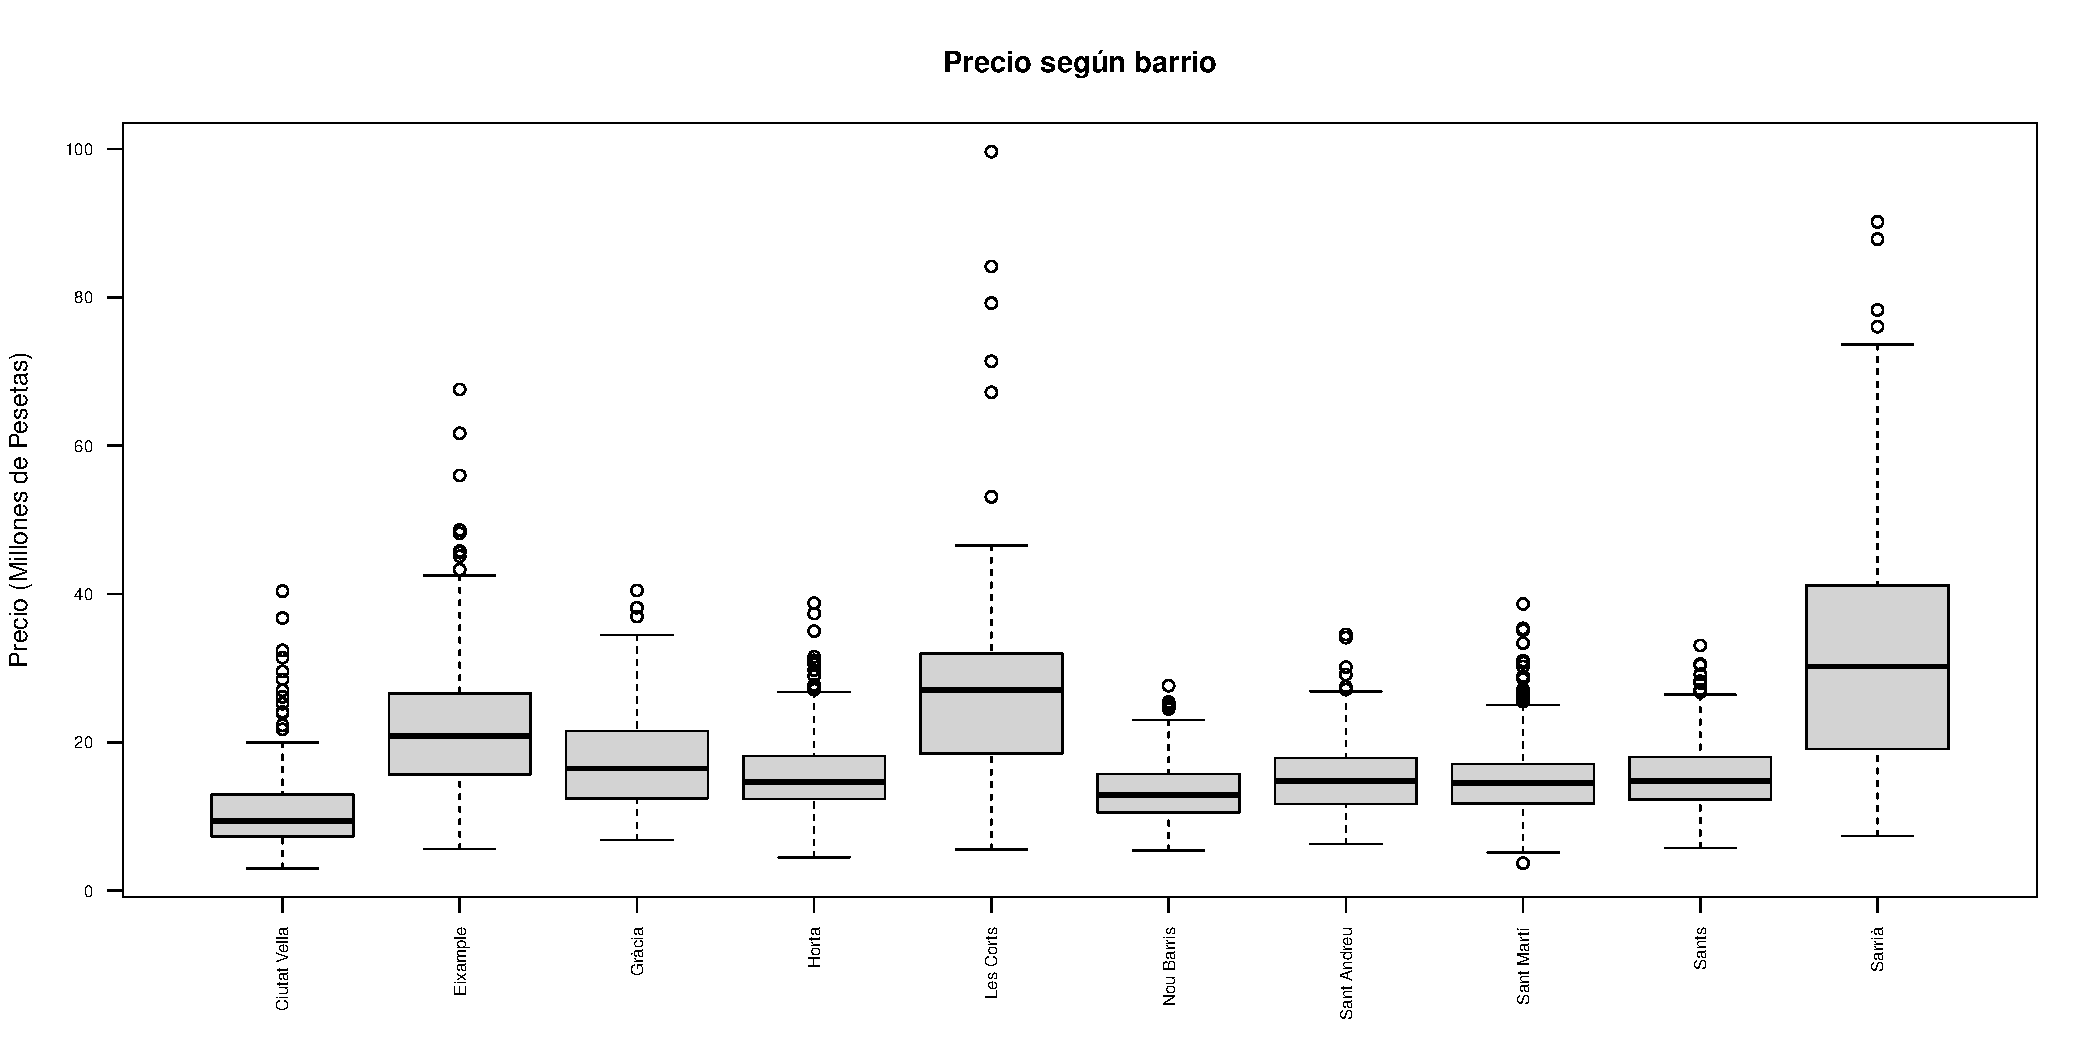
\includegraphics[width = \linewidth]{pr1_boxplot2.pdf}
\end{figure}
Al ser una variable categórica y otra contínua, el test que hay que hacer para determinar la independencia de las variables es la F de \textit{Fisher}.
\begin{equation*}
    \begin{cases}
        H_0 : \text{Valor y Dist son independientes} \\
        H_1 : \text{Valor y Dist no son independientes}
    \end{cases}
\end{equation*}

\begin{rcode}
> oneway.test(pisos_so$Valor ~ pisos_so$Dist, var.equal = TRUE)

        One-way analysis of means

data:  pisos_so$Valor and pisos_so$Dist
F = 121.97, num df = 9, denom df = 2242, p-value < 2.2e-16
\end{rcode}

Con el \textit{p-value} tan pequeño, hay que descartar la hipótesis nula $H_0$
y aceptar que el distrito y el valor de los pisos están relacionados.

\newpage

\begin{tcolorbox}[colback=gray!20,colframe=gray!20, sharp corners]
10. Calcule la asociación entre el “Distrito” y el “Estado de la vivienda”.
\end{tcolorbox}


\begin{table*}[h]
    \centering
    \small
    \begin{tabular}{lrrrrrr}
        
        Distrito & Muy malo & Malo & Normal & Bueno & Muy bueno & $N_j\ (f_j)$ \\
        \midrule
        Ciutat Vella & 74 & 52 & 45 & 9 & 6 & 186 (0.08) \\
        Eixample & 76 & 119 & 119 & 35 & 18 & 367 (0.16) \\
        Gràcia & 36 & 49 & 49 & 23 & 5 & 162 (0.07) \\
        Horta & 24 & 68 & 110 & 34 & 13 & 249 (0.11) \\
        Les Corts & 4 & 26 & 36 & 11 & 6 & 83 (0.04) \\
        Nou Barris & 29 & 77 & 94 & 17 & 6 & 223 (0.10) \\
        Sant Andreu & 19 & 53 & 84 & 19 & 10 & 185 (0.08) \\
        Sant Martí & 45 & 89 & 119 & 55 & 17 & 325 (0.14) \\
        Sants & 42 & 95 & 121 & 41 & 20 & 319 (0.14) \\
        Sarrià & 19 & 51 & 56 & 22 & 5 & 153 (0.07) \\
        \midrule
        $N_i\ (f_i)$ & 368 (0.16) & 679 (0.30) & 833 (0.37) & 266 (0.12) & 106 (0.05) & 2251 (1.00) \\
        
    \end{tabular}
\end{table*}

Con una variable categórica nominal y una categórica ordinal, hemos visto la tabla de contingencia, vamos a aplicar el test estadístico sobre las hipótesis
\begin{equation*}
    \begin{cases}
        H_0 : \text{Dist y Estat son independientes} \\
        H_1 : \text{Dist y Estat no son independientes}
    \end{cases}
\end{equation*}
\begin{rcode}
 > chisq.test(pisos_so$Dist, pisos_so$Estat)

        Pearson's Chi-squared test

data:  pisos_so$Dist and pisos_so$Estat
X-squared = 151.29, df = 36, p-value = 4.407e-16
\end{rcode}

El p-value es muy pequeño, por lo que tenemos que rechazar la hipótesis nula y aceptar que el estado de la vivienda y el distrito tienen una relación estadísticamente significativa.
\end{document}

